To identify the behaviour of the transverse conductivity of the quantum Hall systems with external dressing field we can derive a expression for a normalized
transverse conductivity as a function of fermi energy $X_F$ and intensity of the dressing field $I$. Here we have normalized the conductivity using the natural conductivity of least Landau level.
\begin{equation} \label{eq_36}
  \begin{aligned}
    \sigma^{xx}(X_F,I) = &
    \sum_{n}
    \frac{\qty(n+1)}{0.0037\Lambda_n \Lambda_{n+1}} \\
    & \times
    \qty[
      \frac{1}
      {
        1 + \qty(\frac{X_F - n -1}{0.06\Lambda_n})^2
      }
    ]
    \qty[
      \frac{1}
      {
        1 + \qty(\frac{X_F - n}{0.06\Lambda_{n+1}})^2
      }
    ]
  \end{aligned}
\end{equation}
Using above expression we can analyse the changes can be done to the transverse conductivity in 2DEG using external dressing field. As given in Fig.~\ref{fig:8.1} and \ref{fig:8.2} we can manipulate the transverse conductivity $\sigma_{xx}$ using external dressing field's intensity and the Fermi level $X_F$ of the considering system. When the applied field's intensity increase the broadening of energy bands of Landau levels get reduced and simulaniously the transverse conductivity also get low value for all the regions except the peak point of the energy band. Using this manipulation we can make more narrow or wide the conductivity regions. Since Fermi level of the system can be change with the applied gate voltage of the material this can be used as a 2D switch for optoelectonic applications \cite{dini16}. Controlling  the external dressing field we are able to fine-tune the switching mechanism for optimized performance.
\begin{figure}[t]
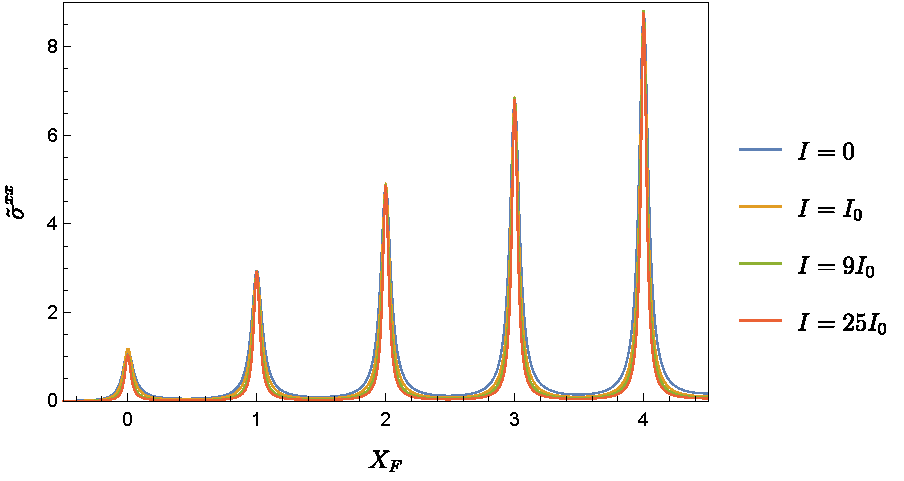
\includegraphics[scale=0.55]{figures/fig_5}
\caption{\label{fig_1} Normalized transverse conductivity $\sigma_{xx}$ against Fermi level $X_F$ with different intensities $I$ of the external dressing field in a GaAs-based quantum well at a magnetic field $B = 1.2~\text{T}$, dressing field with frequency $\omega =2\times10^{12}~\text{rad}\text{s}^{-1}$. In this calculation we have assumed that the natural  broadening of $0$-th Landau level $\Gamma_0$ is $0.24\;\text{me}V$.}
\end{figure}
\begin{figure}[t]
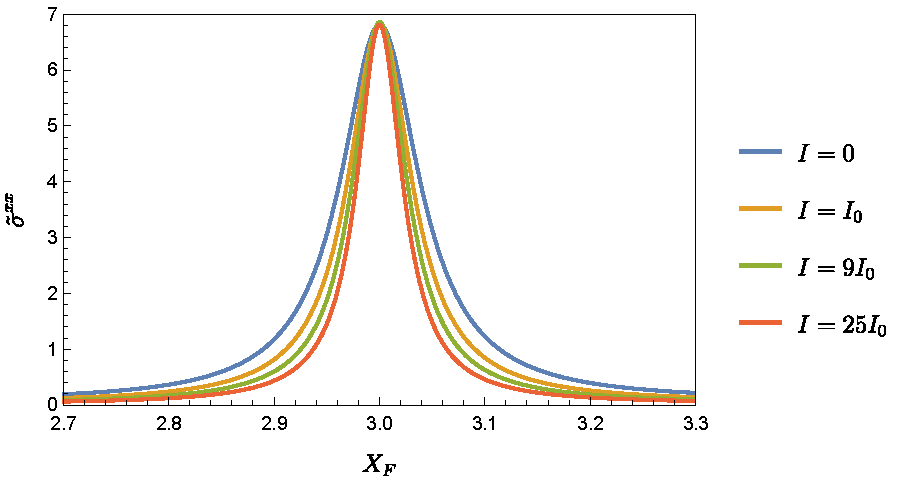
\includegraphics[scale=0.55]{figures/fig_6}
\caption{\label{fig_1} $3$rd Landau level’s normalized transverse conductivity $\sigma_{xx}$ against Fermi level $X_F$ with different intensities $I$ of the external dressing field in a GaAs-based quantum well at a magnetic field $B = 1.2~\text{T}$, dressing field with frequency $\omega =2\times10^{12}~\text{rad}\text{s}^{-1}$ and intensity $I =100~\text{W}/\text{cm}^{2}$. In this calculation we have assumed that the natural  broadening of $0$-th Landau level $\Gamma_0$ is $0.24\;\text{me}V$}.
\end{figure}
